In this Section we detail the process of gathering data from human
subjects and the processing that makes them suitable for
analysis by a machine learning system. In particular, we address the
problem of building a \emph{training set}, that is, a set of data
effectively representing, for each user and object considered, the
grasping process, that could be used to train the system.

\subsection{Experimental Setup}

\subsubsection*{Devices}

We collected data using a $22$-sensors Immersion CyberGlove for the
hand posture \cite{cyberglove}, an Ascension Flock-Of-Birds (FoB) for
the hand position \cite{fob} and a Force Resistor Sensor (FSR) to
detect the contact moment with the object. Figure \ref{fig:devices}
shows the devices, as worn by a subject.

\begin{figure}[htbp]
  \begin{center}
    \begin{tabular}{cc}
      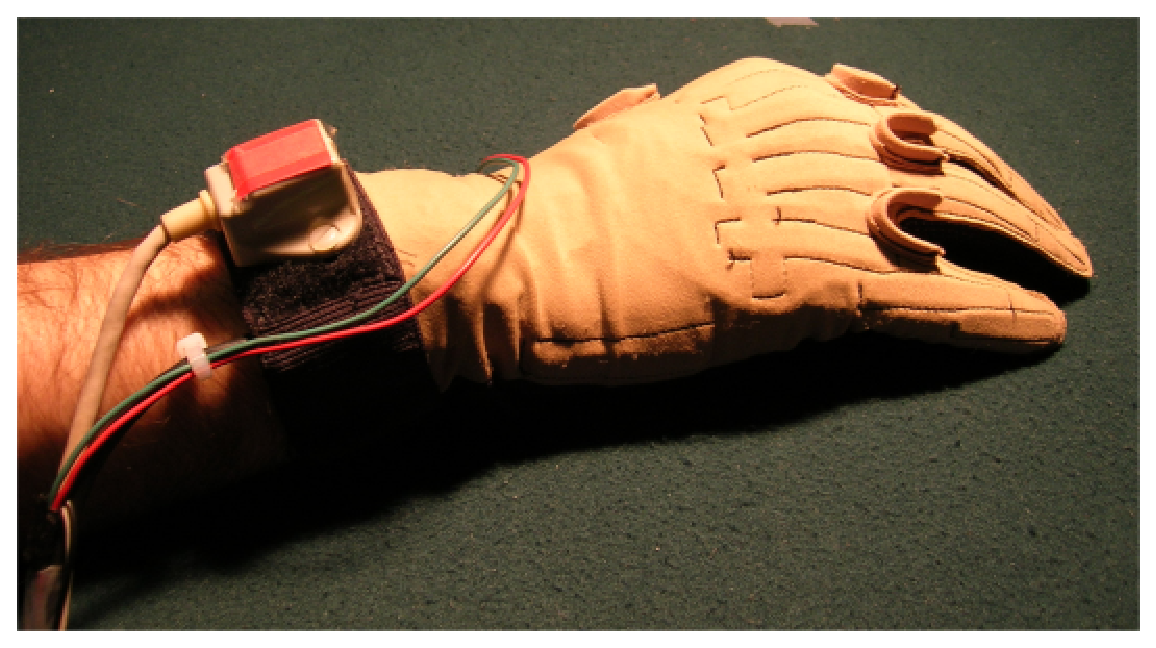
\includegraphics[width=0.45\linewidth]{devices1.eps} &
      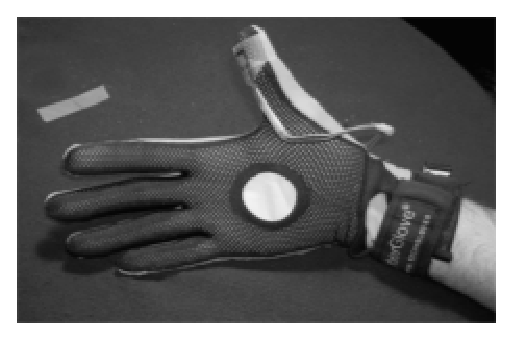
\includegraphics[width=0.45\linewidth]{devices2.eps} \\
      $(a)$ & $(b)$
    \end{tabular}
    \caption{The devices used for the experiment, as worn by a
    subject: $(a)$ the CyberGlove, with the Flock-of-Birds just above
    the subject's wrist; $(b)$ the Force Resistor Sensor attached to
    the subject's thumb.}
    \label{fig:devices}
  \end{center}
\end{figure}

The CyberGlove was worn by the subject on the right hand. The device
returns $22$ $8$-bit numbers linearly related to the angles between
the ends of the sensors and roughly indicating the angles between the
subject's hand joints; the sensors are embedded in the glove in order
for them to be adherent to the subject's skin. The resolution of the
sensors is on average about $0.5$ degree \cite{cyberglove}, but the
noise associated with the sensors has been experimentally determined
to be $1.1$ on average and $3$ at the maximum \cite{212431}. The
sensors describe the position of the three phalanxes of each finger
(for the thumb, rotation and two phalanxes), the four finger-to-finger
abductions, the palm arch, the wrist pitch and the wrist yaw.

The FoB was firmly mounted on the CyberGlove, just above the subject's
wrist, with the $X/Y$ plane being parallel to the palm plane in the
resting position. The device returns $6$ double-precision numbers
describing the position ($x$, $y$ and $z$ in inches) and rotation
(azimuth, elevation and roll in degrees) of the sensor with respect to
a magnetic basis mounted about one meter away from the subject. The
FoB's resolution is $0.1$ inches and $0.5$ degrees \cite{fob}.

Lastly, the FSR was mounted on the subject's thumb. It returns a
$32$-bit number approximately inversely proportional to the pressure
applied to the surface of the sensor. We only used the FSR as an
on-off indicator of when the subject made contact with the object.

All data were collected, synchronised, and saved in real time at a
frequency of $50$Hz.

\subsubsection*{Subjects}

Eleven subjects, four females and seven males aged $24$ to $34$ of
different nationalities, joined the experiment. They were all
right-handed and fully able-bodied, and were given initially some
knowledge of the aim of the experiment.

\subsubsection*{Method}

The subjects were asked to sit comfortably in front of a clean
workspace of about one square meter, at the center of which an object
was placed, in a predefined position. The subjects were then asked to
wear the devices and choose a resting position for their right hand
and arm. They were then instructed to grasp the object with their
right hand as they felt appropriate, not necessarily the same way each
time, keeping a ``natural'' attitude. After grasping the object, they
had to drop it somewhere else in the workspace, and then return their
right hand and arm in the initial resting position. Subsequently, they
had to use their left hand to reposition the object roughly in the
same place it was before.

We first had the subjects do a trial run of the experiment, in order
for them to gain confidence in the setup. A beeping sound was heard
each time the subject made contact with the object (that is, each time
the FSR signalled a significant change), and they were asked to try
and hear the beep each time they grasped the object. Although this
ruled out grasps which made no use of the thumb, it enabled us to
better determine the contact points.

After the trial run, subjects were asked to repeat the
grasp/drop/reposition procedure $120$ times for each object. We will
call both this procedure and the data time sequence gathered during
the procedure, a \emph{session}. We employed, in turn, three objects:
a beer can, a duct tape roll and a mug (Figure \ref{fig:objects}
shows the objects). The objects were chosen so that each of them could be
grasped in several different ways, but with a certain degree of
overlapping, e.g., both the beer can and the mug could be grasped
cylindrically, but only the mug could be grasped using the handle.

\begin{figure}[htbp]
  \begin{center}
    \begin{tabular}{ccc}
      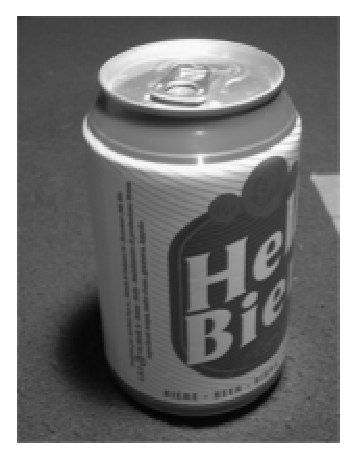
\includegraphics[height=0.2\textheight]{beer.eps} &
      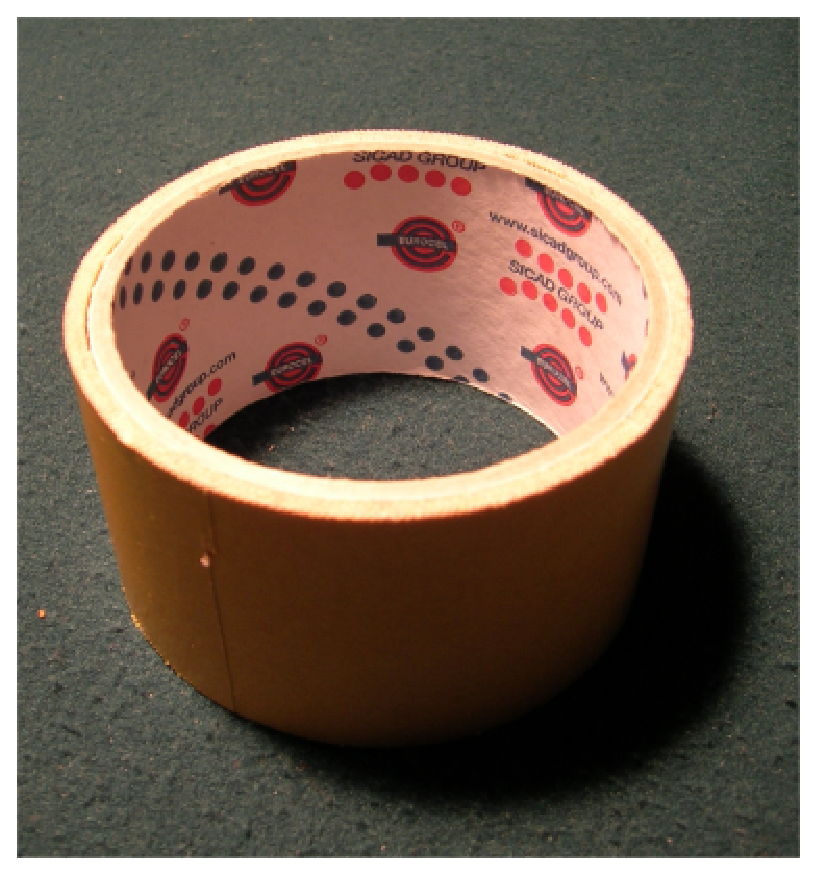
\includegraphics[height=0.2\textheight]{scotch.eps}  &
      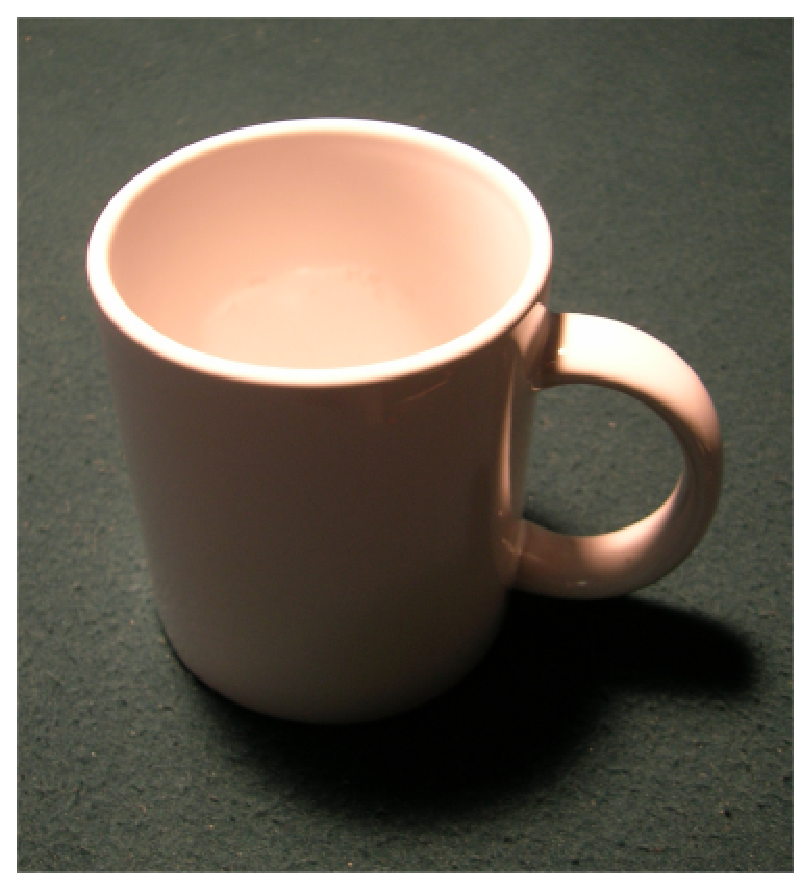
\includegraphics[height=0.2\textheight]{mug.eps} \\
      $(a)$ & $(b)$ & $(c)$
    \end{tabular}
    \caption{The objects used in the experiment: a beer can $(a)$, a
    duct tape roll $(b)$ and a mug $(c)$.}
    \label{fig:objects}
  \end{center}
\end{figure}

Each experiment employed one subject and consisted of six sessions:
first the can, then the roll and then the mug, all of them twice,
for an approximate total of $720$ grasps per subject, $240$ per
object. The numbers are not precise since now and then the subjects
would grasp without properly activating the FSR. This problem has been
corrected in the batch analysis of the data.

Each experiment lasted $35$ to $56$ minutes depending on the subject's
confidence and speed; although almost no subjects reported tiredness,
we allowed them to rest between sessions. It was reported by almost
every subject that the experiment became rapidly boring, which lets us
claim that almost all grasps were done in a natural way, almost
unconsciously. Figure \ref{fig:setup} shows the main phases of the
experiment.

\begin{figure}[htbp]
  \begin{center}
    \begin{tabular}{ccc}
      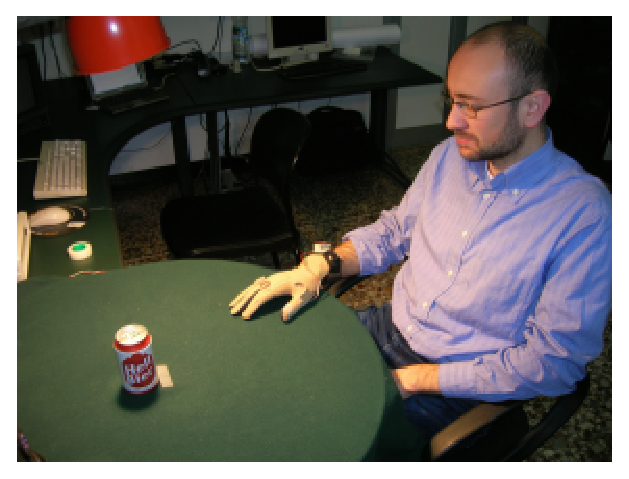
\includegraphics[width=0.3\linewidth]{exp1.eps} &
      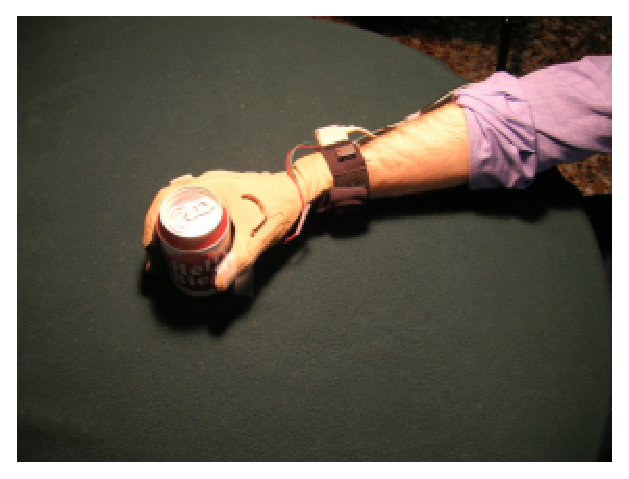
\includegraphics[width=0.3\linewidth]{exp2.eps}  &
      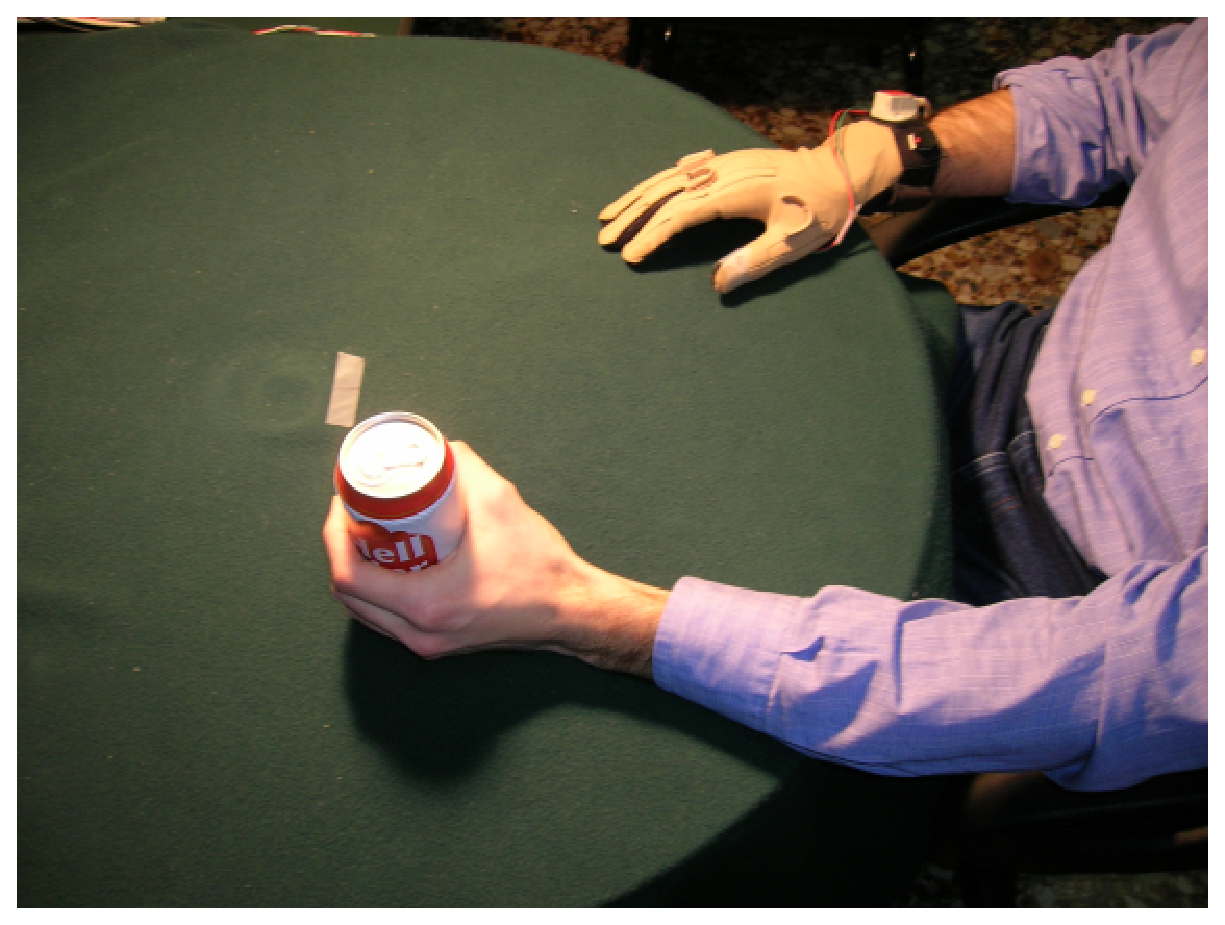
\includegraphics[width=0.3\linewidth]{exp3.eps} \\
      $(a)$ & $(b)$ & $(c)$
    \end{tabular}
    \caption{The experiment. The subject sits comfortably in front of
    a clean workspace, at the center of which an object is placed
    $(a)$, with his right hand in a resting position. He then grasps
    the object and drops it somewhere else in the workspace $(b)$,
    bringing then his arm and hand in the resting position. Lastly, he
    repositions the object in the initial position using his left arm
    and hand $(c)$.}
    \label{fig:setup}
  \end{center}
\end{figure}

\subsection{Building the training set}

\subsubsection*{Detecting grasps}

In order to figure out when each single grasp starts and ends in a
session, we first observed the values of the FSR mounted on the
subject's thumb. We manually verified that the FSR correctly reacted
in almost all cases with a spike, signalling, whenever the subject
made contact with the object, a significantly different value from
that recorded elsewhere shortly before the contact. The spike instants
were taken as the \emph{ending} points of each grasp, and were
gathered by checking when the first derivative of the FSR value
dropped by more than $10\%$ of its overall minimum value. Moreover,
after each spike, we ignored one second of the session, to avoid 
detecting possible spurious spikes which happened immediately after
the grasp, due to object slippage and/or blurred values coming from
the FSR.

Subsequently, in order to detect the \emph{starting} point of each
action, for each ending point we observed the hand speed and
acceleration, averaged over $0.2$ seconds, from the ending point
backwards. Since we had instructed the subjects to always return to
the resting position before initiating a new grasp, when the grasp
starts, the speed must be close to zero and the acceleration must be
negative (the subject's arm is moving \emph{toward} the FoB's
reference point). Therefore, we set the grasp starting point at the
nearest moment in time before the ending point in which the hand speed
was close to zero and the hand acceleration was negative. In order to
avoid detecting spurious speed/acceleration glitches when the hand
made contact with the object, we ignored $0.1$ seconds just before the
ending point; moreover, we ignored grasps which resulted shorter than
$280$ milliseconds. All these values were determined experimentally to
be near optimal in order to catch as many grasps as possible while
avoiding spurious ones.

Figure \ref{fig:grasp_sequence} $(a)$ shows an example set of detected
grasps. As one can see, the hand speed (green curve) shows the well
known bell-shaped profile of a planar reaching movement \cite{morasso-81}: 
the hand acceleration diminishes, changes sign and then goes back to zero at 
the end of the trajectory.

\begin{figure}[htbp]
  \begin{center}
    \begin{tabular}{ccc}
      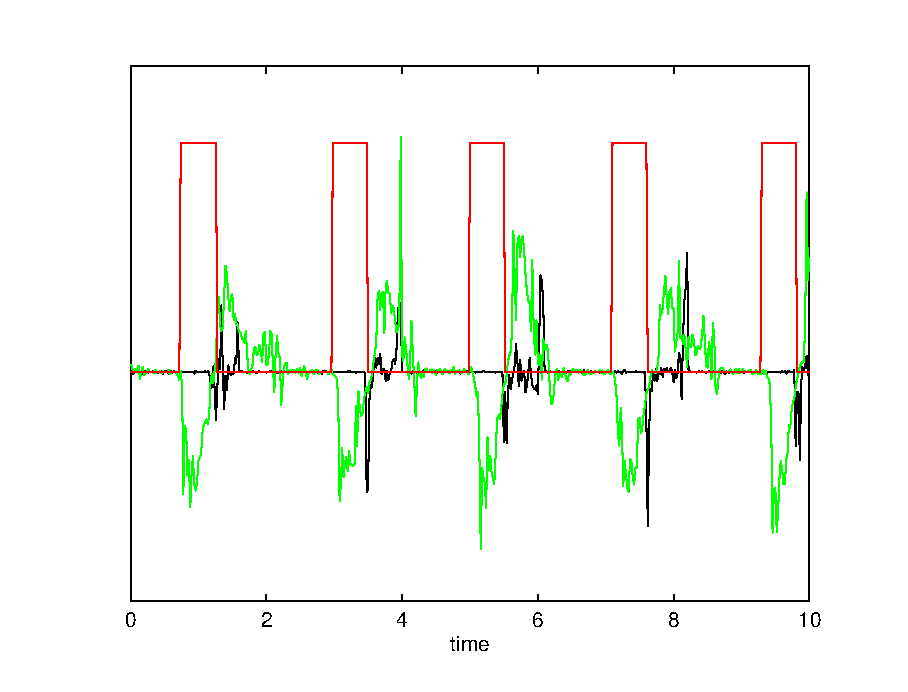
\includegraphics[width=0.48\linewidth]{grasp_seq_scotch.eps} &
      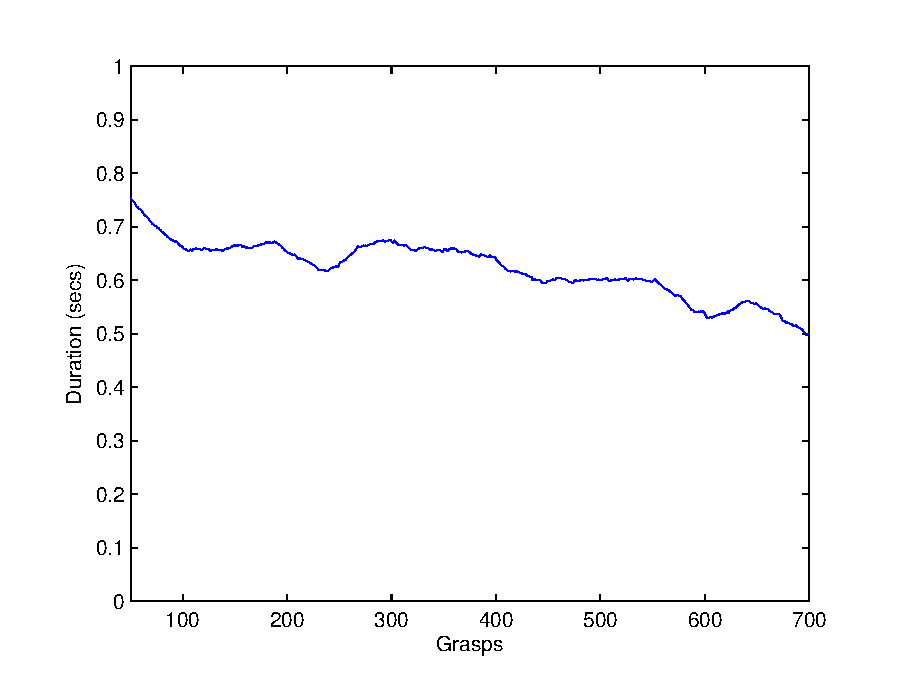
\includegraphics[width=0.48\linewidth]{grasp_trend.eps} \\
      $(a)$ & $(b)$
    \end{tabular}
    \caption{$(a)$ Detecting the grasps. The Figure shows $10$ seconds
    of a subject grasping an object. The red bands indicate the start
    and end of a grasp; the black line is the FSR response; and the
    green line is the hand speed. As one can see, the ending points
    are found near the FSR spike, indicating contact; moreover, the
    hand speed shows the well known bell-shaped profile of planar
    reaching \cite{morasso-81}. 
    $(b)$ Grasps duration. The Figure shows the duration of the
    grasps (moving average over $50$ grasps) averaged for all
    subjects. As the experiments advance, the duration becomes shorter.}
    \label{fig:grasp_sequence}
  \end{center}
\end{figure}

Overall, the procedure could recognise $716 \pm 12$ grasps for each
subject, which matches the desired result of $720$, that is $120$ per
session, each user running six sessions (during two experiments, the
FSR sensor broke down, resulting in the recognition of only $550$ and
$649$ grasps). All data were also parsed by hand in order to verify
that spurious detected grasps would be an insignificant fraction of
the total grasps.

\subsubsection*{The blind window}

In order to test the power of prediction of our machine, we needed to
somehow \emph{hide} to the system the final part of the grasping
action. We therefore defined a \emph{blind window} $B$, with $0
\leq B \leq 1$, representing what fraction of the grasp, from the
contact point backwards, was hidden. Figure \ref{fig:B_example} shows a
typical situation. It was intuitively expected that larger values of
$B$ would smoothly lead to larger errors.

\begin{figure}[htbp]
  \begin{center}
    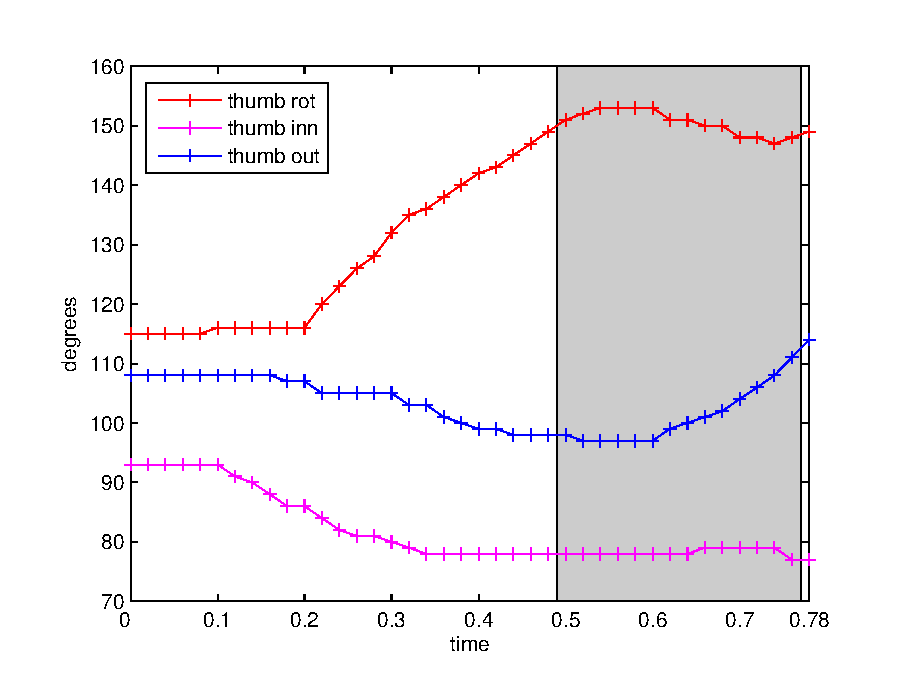
\includegraphics[width=0.5\linewidth]{B_example.eps}
    \caption{The blind window (the grey zone in the Figure) indicates
    what fraction of each grasp, from the contact point backwards, is
    hidden to the learning machine.
    The data shown is a typical trajectory of the
    thumb (rotation, inner phalanx, outer phalanx) during a grasp. In
    this case the grasp lasts $0.78$ seconds and $B=0.375$. The last
    sample (for $t=0.78$) is the target value.}
    \label{fig:B_example}
  \end{center}
\end{figure}

Moreover, in general, in order to make time sequences suitable for
regression, they all must have the same length\footnote{An alternative
possibility appears, e.g., in \cite{shimodaira02dynamic}; this issue
is the subject of future research.} so that they can be represented as
vectors in a fixed-dimension input space. In order to accomplish this,
since in general not all grasps have the same length, for each grasp
we decided to stretch its \emph{visible} window (i.e., a fraction of
the grasp corresponding to $1-B$) to a predefined length; and it
seemed reasonable to choose this length according to the average speed
of the grasps, in order not to lose any information.

Figure \ref{fig:grasp_sequence} $(b)$ shows the average grasp
durations for all subjects over each experiment (moving average over
$50$ grasps); as one would expect, in general the subjects get rapidly
used to the grasp/drop/reposition task and the grasps become faster
and faster. It must be remarked, though, that this is not the case for
all subjects when considered individually. On average, the grasp
duration was $0.62 \pm 0.20$ seconds. We decided then to stretch every
visible window to $1$ second by linear interpolation, obtaining
fixed-length time sequences of $50$ samples for each sensor and grasp;
these time sequences were then represented as vectors in a
$50$-dimensional space.

\subsection{Support Vector Machines}

Our machine learning system is based upon Support Vector Machines
(SVMs). Introduced in the early 90s by Boser, Guyon and Vapnik
\cite{BGV92}, SVMs are a class of kernel-based learning algorithms
deeply rooted in Statistical Learning Theory \cite{v-edbed-82}, now
extensively used in, e.g., speech recognition, object classification
and function approximation with good results \cite{Cristianini00}. We
now give a very quick account of SVMs; for an extensive introduction
to the subject, see, e.g., \cite{SmolaTut2004}.

We are interested here in the problem of SVM regression, that is:
given a function whose value is known only for a finite number of
points in its input domain, find its best approximation $f$ drawn from
a suitable functional space $\mathcal{F}$. In practice, let
$S=\{\xx_i,y_i\}_{i=1}^l$, with $\xx_i \in \RR^m$ and $y_i \in \RR$ be
a set of $l$ points and output values of the unknown function
(actually, the training set); then the resulting $f(\xx)$ is a sum of
$l$ elementary functions $K(\xx,\yy)$, each one centered on a point in
$S$, and weighted by real coefficients $\alpha_i$:

\begin{equation} \label{eqn:sol}
  f(\xx) = \sum_{i=1}^l \alpha_i K(\xx,\xx_i) + b
\end{equation}

\noindent where $b \in \RR$. The choice of $K$, the so-called
\emph{kernel}, is done \emph{a priori} and defines $\mathcal{F}$
once and for all; it is therefore crucial. According to a standard
practice (see, e.g., \cite{Cristianini00}) we have chosen a
\emph{Gaussian} kernel, so that

\begin{equation} \label{eqn:ker}
  K(\xx,\yy) = e^{-\frac{||\xx-\yy||^2}{\sigma^2}}
\end{equation}

\noindent where $\sigma \in \RR^{+}$ is the \emph{standard deviation} of
the Gaussian function $K$.

Now, let $C \in \RR$ be a positive number; then the $\alpha_i$s and
$b$ in (\ref{eqn:sol}) are found by solving the following minimisation
problem (\emph{training phase}):

\begin{equation} \label{eqn:svm_primal}
  \min \left( R(S,K,\aa) + C \sum_{i=1}^l L^\epsilon (\xx_i,y_i,f) \right)
\end{equation}

\noindent where $R$ is a \emph{regularisation term} and
$L^\epsilon$ is a \emph{loss functional}. Minimising the sum of $R$
and $L^\epsilon$ together ensures that the solution will approximate
well the values in the training set (thanks to $L^\epsilon$), at the
same time avoiding overfitting, i.e., exhibiting poor accuracy on
points outside $S$ (thanks to $R$). The regularisation term actually
controls the ``complexity'' of $f(\xx)$. As is apparent from
(\ref{eqn:svm_primal}), $C$ balances the relative importance of
$L^\epsilon$ and $R$. In SVM regression, it is usually the case that
$L^\epsilon (\xx_i,y_i,f) = \mbox{max}(0,|y_i-f(\xx_i)|-\epsilon)$,
where $\epsilon > 0$ controls the width of an ``insensitive band''
around the output values, e.g., errors on the training set within this
band are not considered.

In the end, there are three numbers to be tuned in our setting, called
\emph{hyperparameters}: $C$, $\sigma$ and $\epsilon$. In all our
regression tests, we found the optimal values of $C$ and $\sigma$ by
grid search with $5$-fold cross-validation, whereas $\epsilon$ was
chosen accordingly to the resolution of the sensors being examined
(see next Section for a more detailed discussion). This is standard
practice in the machine learning literature.

It is also usually the case that, after the training phase, some of
the $\alpha_i$s are found to be zero; the $\xx_i$s associated with
non-zero $\alpha_i$s are called \emph{support vectors} (SVs). Both the
training time (i.e., the time required by the training phase) and the
testing time (i.e., the time required to find the value of a point not
in $S$) crucially depend on the total number of SVs; therefore, the
total number of SVs is an indicator of how hard the problem is. An
even better indicator is the \emph{fraction} of SVs with respect to
$|S|$, since in the standard SVM setting the number of SVs grows
proportionally to the total number of samples in $S$
\cite{Steinwart03}.

Notice, lastly, that the quantity to be minimised in Equation
(\ref{eqn:svm_primal}) is convex; due to this, as well as to the use
of a kernel, SVMs have the advantages that their training is
guaranteed to end up in a global solution and that they can easily
work in highly dimensional, non-linear feature spaces, as opposed to
analogous algorithms such as, e.g., artificial neural networks. Our
system employs LIBSVM v2.82 \cite{ChangL01}, a standard, efficient
implementation of SVMs.

According to the procedure described in the previous parts of this
Section, we defined $\RR^{50}$ as the input space of our machines. We
have then set up $28$ such SVMs, each one approximating the value of a
sensor at the time of contact.
